\section{Características}
	Por ser um SGBD NoSQL distribuído, o Amazon SimpleDB não possui algumas garantias que são encontradas em SGBDs relacionais não-distribuídos. Em princípio, seria desejável obter um sistema que garantisse as seguintes propriedades:
\begin{itemize}
	\item
	\textbf{Disponibilidade}: o sistema deve continuar utilizável mesmo que alguns dos nós que o compõem falhem;
	
	\item
	\textbf{Tolerância a particionamento}: se alguns nós do sistema perderem o contato entre si na rede que os interconecta, o sistema deve continuar operacional;
	
	\item
	\textbf{Consistência}: Os dados presentes em um nó que compõe o banco não devem entrar em conflito com os dados em outro nó.
\end{itemize}

	O teorema CAP, no entanto, assevera que é impossível que um sistema distribuído apresente as três propriedades relacionadas acima ao mesmo tempo\cite{WikiCapTheo}. O Amazon SimpleDB abre mão da consistência em favor de uma \textit{consistência eventual}: ela apenas assegura que, dado tempo suficiente sem atividades de alteração no banco de dados, eventualmente todas os nós do banco estarão consistentes entre si\cite{WikiEvCons}.\\
	A API do serviço permite que a aplicação cliente especifique diferentes graus de consistência(leituras consistentes, semântica transacional, etc) ao realizar operações sobre o banco. Tais exigências, no entanto, pioram a performance do acesso ao serviço e devem ser usadas somente quando necessárias.
	
\subsection{Limites}
O serviço possui as seguinte limitações\cite{WikiSimpleDb}:
\begin{itemize}
	\item máximo de 250 domínios por conta;
	\item máximo de 10GB em cada domínio;
	\item máximo de 1 milhão de atributos por domínio;
	\item máximo de 256 atributos por item;
	\item máximo de 1KB por atributo;
	\item máximo de 2500 itens retornados por consulta;
	\item timeout de 5 segundos por consulta;
	\item no máximo 1 atributo referenciado em cada predicado de consulta;
	\item máximo de 22 operadores em cada predicado de consulta;
	\item máximo de 20 predicados em cada consulta.
\end{itemize}

\subsection{Modelo de dados}
	O Amazon SimpleDB difere-se de um SGBD relacional convencional principalmente no fato de não organizar os dados em tabelas, mas sim em \textbf{domínios}. Estes, por sua vez, são compostos por \textbf{itens} com nomes únicos que agrupam um conjunto de \textbf{atributos}, cada um consistindo num par chave-valor, sendo que todo atributo possui um índice criado automaticamente pelo sistema. Deve-se ressaltar que um atributo pode ter múltiplos valores(o seu valor é um vetor). Essa organização se encontra ilustrada na figura \ref{fig:hierarquiaDados}. Os itens em um mesmo domínio não precisam ter os mesmos atributo e todos os atributos são opcionais(isto é, aceitam valores vazios).
\begin{figure}
	\centering
	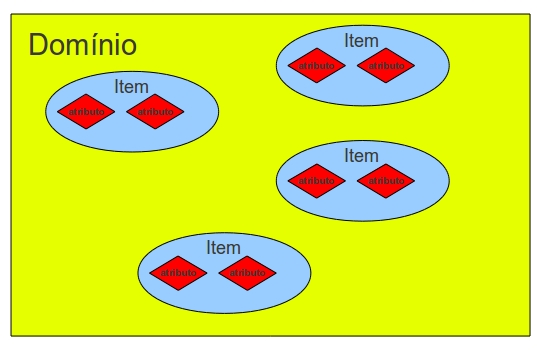
\includegraphics[scale=0.5]{figuras/simpledb_hierarquia_dados.jpg}
	\label{fig:hierarquiaDados}
	\caption{Modelo de dados do Amazon SimpleDB}
\end{figure}
\\\\ Os valores são armazenados como strings independentemente do seu tipo - fica a cargo da aplicação cliente fazer as conversões e operações de \textit{marshalling} necessárias. Uma consequência desse fato é que o programador deve ter cuidado para converter os tipos de forma que operações de comparação mantenham-se consistentes. Valores numéricos devem ser completados com zeros à esquerda para evitar que, por exemplo, o número 123 seja classificado como anterior ao número 54(já que, lexicograficamente, esso é o comportamento esperado); caso se deseje trabalhar com números negativos, deve-se adicionar um offset ao número armazenado e, quando ele for requisitado, o offset deve ser subtraído para se obter o valor original; datas devem ser convertidas para formatos que preservem ordenamento lexicográfico, como o ISO 8601 define.
\\\\ Uma diferença fundamental entre SGBDs relacionais e o Amazon SimpleDB é a ausência de suporte a operações de \textit{joins} neste último. Se o modelo de dados utlizados na aplicação cliente contém dados relacionados entre si, a própria aplicação deve implementar algum mecanismo para agregar entradas de dados relacionadas (ou usar um SGBD relacional ao invés de uma opção NoSQL). Note que essa abordagem pode levar a um modelo de dados \textit{não-normalizado} --- isso, porém, faz parte do tradeoff envolvido no uso de soluções NoSQL: abre-se mão da normalização de dados e restrições de consistência em favor de performance, escalabilidade e simplicidade.